% !TEX program = xelatex
% AY2020 材料力学 解答例（同志社 生命医科学 医工学コース 院試）
% 問題・図は 01_exams/2020/tex を土台に、参考/ の粒度で解答を付した。
\documentclass[11pt,a4paper]{article}
\usepackage{../../00_common/preamble}
\usetikzlibrary{positioning,arrows.meta,calc,patterns,decorations.pathmorphing}

\title{材料力学 AY2020 解答例（専門応用科目）}
\author{}
\date{}

\begin{document}
\maketitle

\noindent\textbf{符号規約}：軸力 $N$ は引張りを正，座標 $x$ は右向き（はりでは固定端 A から）を正，
変位・たわみは座標正の向き（軸方向は右向き，はりでは上向き）を正とする．
せん断力 $Q$ は断面左側に働く上向き外力の和，曲げモーメント $M$ は下に凸（さがり）を正とし，
たわみの基礎式は $EI\,\dfrac{d^2v}{dx^2}=M(x)$ を用いる．

%====================================================================
\section*{〔I〕}

図1に示すように, 棒\textcircled{1}, 棒\textcircled{2}からなる段付き棒の両端を固定し, 棒\textcircled{1}には外力 $P_1$,
棒\textcircled{2}には外力 $P_2$ を加えた. 棒\textcircled{1}, 棒\textcircled{2}の長さは共に $L$, 断面積はそれぞれ $A$ および $2A$,
縦弾性係数は $3E$ および $E$ とする.

\begin{center}
\begin{tikzpicture}[>=Latex]
  \fill[pattern=north east lines] (-0.5,-1.3) rectangle (0,1.0); \draw (0,-1.3) -- (0,1.0);
  \fill[pattern=north east lines] (8,-1.3) rectangle (8.5,1.0); \draw (8,-1.3) -- (8,1.0);
  \draw (0,0.5) rectangle (4,-0.5);
  \draw (4,0.8) rectangle (8,-0.8);
  \draw[->,very thick] (2,0) -- (1.1,0); \node[above] at (1.7,0.05) {$P_1$};
  \draw[->,very thick] (5.33,0) -- (6.3,0); \node[above] at (5.9,0.05) {$P_2$};
  \node at (3.1,0.25) {棒\textcircled{1}}; \node at (3.1,-0.25) {\footnotesize $A,\,3E$};
  \node at (6.9,0.35) {棒\textcircled{2}}; \node at (6.9,-0.1) {\footnotesize $2A,\,E$};
  \node[below] at (0,-1.45) {a}; \node[below] at (2,-1.45) {b}; \node[below] at (4,-1.45) {c};
  \node[below] at (5.33,-1.45) {d}; \node[below] at (8,-1.45) {e};
  \draw[<->] (0,1.2) -- (4,1.2) node[midway,fill=white]{$L$};
  \draw[<->] (4,1.2) -- (8,1.2) node[midway,fill=white]{$L$};
  \draw[<->] (2,-0.78) -- (4,-0.78) node[midway,fill=white,inner sep=1pt,font=\scriptsize]{$L/2$};
  \draw[<->] (4,-1.08) -- (5.33,-1.08) node[midway,fill=white,inner sep=1pt,font=\scriptsize]{$L/3$};
\end{tikzpicture}

\vspace{1mm}
図1
\end{center}

\begin{enumerate}[label=(\arabic*)]
  \item 棒\textcircled{1}および棒\textcircled{2}の変位 $\lambda_1$, $\lambda_2$ を求めよ.
  \item c の変位が 0（ゼロ）となる $P_2$ を $P_1$ を用いて表せ.
\end{enumerate}

\subsection*{解答}

両端固定であるから，これは静定では解けない（不静定）問題である．
左壁 a が棒に及ぼす反力を $R_a$，右壁 e が及ぼす反力を $R_e$（ともに $+x$ 向きを正）とおく．
節点位置は a を原点として $a=0,\ b=\tfrac{L}{2},\ c=L,\ d=L+\tfrac{L}{3},\ e=2L$ である．
外力は b 点で $P_1$（左向き，$-x$），d 点で $P_2$（右向き，$+x$）．

\medskip
\noindent\textbf{(1)}\quad まず各区間の軸力（引張り正）を求める．断面の左側にある外力の $+x$ 成分の総和を $S$ とすると，
切断面のつり合いより内力は $N=-S$ となる．区間ごとに左側の外力を数えて
\[
  N_{ab}=-R_a,\quad
  N_{bc}=N_{cd}=-(R_a-P_1)=P_1-R_a,\quad
  N_{de}=-(R_a-P_1+P_2)=P_1-P_2-R_a .
\]
棒\textcircled{1}（区間 a--c，剛性 $3E\!\cdot\!A=3EA$）は a--b と b--c がともに長さ $L/2$ であり，その伸びは
\[
  \lambda_1=\frac{N_{ab}\cdot\frac{L}{2}+N_{bc}\cdot\frac{L}{2}}{3EA}
  =\frac{L}{6EA}\bigl(P_1-2R_a\bigr).
\]
棒\textcircled{2}（区間 c--e，剛性 $E\!\cdot\!2A=2EA$）は c--d が長さ $L/3$，d--e が長さ $2L/3$ であり
\[
  \lambda_2=\frac{N_{cd}\cdot\frac{L}{3}+N_{de}\cdot\frac{2L}{3}}{2EA}
  =\frac{L}{2EA}\Bigl[(P_1-R_a)-\tfrac{2}{3}P_2\Bigr]
  =\frac{L}{6EA}\bigl[3(P_1-R_a)-2P_2\bigr].
\]
両端が固定されているから，棒全体の伸びはゼロでなければならない（適合条件）：
\[
  \lambda_1+\lambda_2=0
  \ \Longrightarrow\
  (P_1-2R_a)+\bigl[3(P_1-R_a)-2P_2\bigr]=0
  \ \Longrightarrow\
  4P_1-5R_a-2P_2=0 .
\]
よって反力は
\[
  R_a=\frac{4P_1-2P_2}{5}.
\]
これを代入すると $P_1-2R_a=\dfrac{4P_2-3P_1}{5}$，$\,3(P_1-R_a)-2P_2=\dfrac{3P_1-4P_2}{5}$ であるから
\[
  \ans{\;\lambda_1=\frac{L\,(4P_2-3P_1)}{30EA},\qquad
        \lambda_2=\frac{L\,(3P_1-4P_2)}{30EA}\;}
\]
（$\lambda_1,\lambda_2$ は $+x$ 向きを正とする伸び．負なら縮みを表す．）

\smallskip
検算：$\lambda_1+\lambda_2=\dfrac{L}{30EA}\bigl[(4P_2-3P_1)+(3P_1-4P_2)\bigr]=0$ となり，両端固定の条件と一致する ✓．

\medskip
\noindent\textbf{(2)}\quad 左壁 a は固定されているから，c 点の変位は a から c までの伸び，すなわち棒\textcircled{1}の伸び $\lambda_1$ に等しい．
これが 0 となる条件は
\[
  \lambda_1=\frac{L\,(4P_2-3P_1)}{30EA}=0
  \ \Longrightarrow\
  4P_2-3P_1=0 .
\]
\[
  \ans{\;P_2=\dfrac{3}{4}P_1\;}
\]
検算：$P_2=\tfrac34 P_1$ のとき $R_a=\dfrac{4P_1-2\cdot\frac34P_1}{5}=\dfrac{P_1}{2}$，
よって $N_{ab}=N_{bc}=-\tfrac{P_1}{2}+P_1$ の総和から $\lambda_1=\dfrac{L}{6EA}\bigl(P_1-2\cdot\tfrac{P_1}{2}\bigr)=0$ となり，c の変位が 0 になる ✓．

%====================================================================
\clearpage
\section*{〔II〕}

図2に示すように, 長さ $2L$ の片持ちはりにおいて, A から $L$ の位置 B に曲げモーメント $M_0$,
$2L$ の位置 C に外力 $P$ を加えた. はりの縦弾性係数を $E$, 断面 2 次モーメントを $I$ とする.

\begin{center}
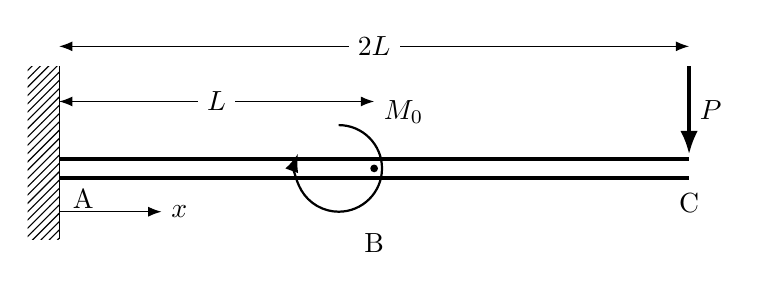
\begin{tikzpicture}[>=Latex]
  \fill[pattern=north east lines] (-0.4,-0.9) rectangle (0,1.3);
  \draw (0,-0.9) -- (0,1.3);
  \draw[line width=1.2pt] (0,0.12) -- (8,0.12);
  \draw[line width=1.2pt] (0,-0.12) -- (8,-0.12);
  \draw[->,thick] (3.55,0.55) arc (90:-200:0.55);
  \node[above right] at (4.0,0.45) {$M_0$};
  \fill (4,0) circle (1.4pt);
  \draw[->,very thick] (8,1.3) -- (8,0.18) node[midway,right]{$P$};
  \node[below right] at (0.05,-0.15) {A}; \node[below] at (4,-0.7) {B}; \node[below] at (8,-0.2) {C};
  \draw[->] (0,-0.55) -- (1.3,-0.55) node[right]{$x$};
  \draw[<->] (0,0.85) -- (4,0.85) node[midway,fill=white]{$L$};
  \draw[<->] (0,1.55) -- (8,1.55) node[midway,fill=white]{$2L$};
\end{tikzpicture}

\vspace{1mm}
図2
\end{center}

\begin{enumerate}[label=(\arabic*)]
  \item せん断力図（SFD）および曲げモーメント図（BMD）を示せ.
  \item B におけるたわみ $\delta_B$ を求めよ.
\end{enumerate}

\subsection*{解答}

片持ちはりであるから，自由端 C 側から数えると反力を求めずに内力が書ける．
固定端を A（$x=0$），B を $x=L$，自由端 C を $x=2L$ とする．
集中モーメント $M_0$ は図の通り時計回りに作用するものとする．

\medskip
\noindent\textbf{(1)}\quad せん断力 $Q(x)$ は断面の左側にある上向き外力の和に等しい．
固定端 A の鉛直反力は，鉛直つり合い $R_A-P=0$ より $R_A=P$（上向き）．
集中モーメント $M_0$ は鉛直力を持たないから，全区間で
\[
  \ans{\;Q(x)=P\qquad(0<x<2L)\;}
\]
曲げモーメントは自由端側の荷重から求める（さがり正）．断面より右側にある荷重のモーメントを数えると，
$x<L$ では右側に $P$（C 点，下向き）と $M_0$（時計回り）があり，$x>L$ では $P$ のみであるから
\[
  M(x)=
  \begin{cases}
    -P(2L-x)-M_0 & (0\le x<L)\\[2pt]
    -P(2L-x)     & (L<x\le 2L)
  \end{cases}
\]
代表値は $M(0)=-2PL-M_0$，$M(L^-)=-PL-M_0$，$M(L^+)=-PL$，$M(2L)=0$．
B 点では集中モーメント $M_0$ により BMD が $M_0$ だけ跳躍する．
\[
  \ans{\;M(x)=\begin{cases}-P(2L-x)-M_0 & (0\le x<L)\\ -P(2L-x) & (L<x\le 2L)\end{cases}\;}
\]

\begin{center}
\begin{tikzpicture}[>=Latex,scale=1.0]
  \def\L{2.6}
  \begin{scope}
    \draw[->] (-0.3,0) -- (2*\L+0.6,0) node[right]{$x$};
    \draw[->] (0,-0.4) -- (0,1.2) node[above]{SFD};
    \draw[line width=1pt,blue] (0,0.7) -- (2*\L,0.7);
    \draw[blue,densely dashed] (0,0)--(0,0.7); \draw[blue,densely dashed] (2*\L,0)--(2*\L,0.7);
    \node[left] at (0,0.7) {$P$};
    \node[below] at (\L,0) {$L$}; \node[below] at (2*\L,0) {$2L$};
    \node[above] at (0,0) {A};
  \end{scope}
  \begin{scope}[xshift=8.5cm]
    \draw[->] (-0.3,0) -- (2*\L+0.6,0) node[right]{$x$};
    \draw[->] (0,-1.5) -- (0,0.6) node[above]{BMD};
    % region1: x=0 -> M=-2PL-M0 (=-1.4), x=L- -> M=-PL-M0(=-0.9)
    \draw[line width=1pt,red] (0,-1.4) -- (\L,-0.9);
    % jump at B: -0.9 -> -PL(=-0.5)
    \draw[line width=1pt,red] (\L,-0.5) -- (2*\L,0);
    \draw[red,densely dashed] (\L,-0.9)--(\L,-0.5);
    \draw[red,densely dashed] (0,0)--(0,-1.4);
    \node[left] at (0,-1.4) {\scriptsize $-2PL-M_0$};
    \node[below right] at (\L,-0.98) {\scriptsize $-PL-M_0$};
    \node[above right=1pt] at (\L,-0.46) {\scriptsize $-PL$};
    \node[above] at (0,0) {A}; \node[below left=-1pt] at (\L,0) {B}; \node[above right] at (2*\L,0) {C};
  \end{scope}
\end{tikzpicture}
\end{center}

\medskip
\noindent\textbf{(2)}\quad たわみの基礎式 $EI\,v''=M(x)$ を固定端側の区間 $0\le x\le L$ で 2 回積分する．
\[
  EI\,v''=M_1(x)=-P(2L-x)-M_0=-2PL+Px-M_0 .
\]
\[
  EI\,v'=-2PL\,x+\frac{P}{2}x^2-M_0\,x+C_1,\qquad
  EI\,v=-PL\,x^2+\frac{P}{6}x^3-\frac{M_0}{2}x^2+C_1x+C_2 .
\]
固定端の境界条件 $v(0)=0,\ v'(0)=0$ より $C_1=C_2=0$．よって
\[
  EI\,v(x)=\frac{P}{6}x^3-PL\,x^2-\frac{M_0}{2}x^2 \qquad(0\le x\le L).
\]
B 点（$x=L$）のたわみは
\[
  EI\,v(L)=\frac{P}{6}L^3-PL^3-\frac{M_0}{2}L^2
  =-\frac{5PL^3}{6}-\frac{M_0L^2}{2}.
\]
\[
  \ans{\;\delta_B=v(L)=-\frac{5PL^3}{6EI}-\frac{M_0L^2}{2EI}
   \quad\Bigl(\text{下向きに }\tfrac{5PL^3}{6EI}+\tfrac{M_0L^2}{2EI}\Bigr)\;}
\]
$P$ と時計回りの $M_0$ はともに B を下向きにたわませるため，両者の寄与は加算される．

\smallskip
検算：$M_0=0$ とすると $\delta_B=-\dfrac{5PL^3}{6EI}$．これは長さ $2L$ の片持ちはりの自由端集中荷重 $P$ による
たわみ式 $v(x)=-\dfrac{Px^2}{6EI}(3\cdot 2L-x)$ に $x=L$ を代入した値
$-\dfrac{PL^2}{6EI}(6L-L)=-\dfrac{5PL^3}{6EI}$ と一致する ✓．

\end{document}
